\section{Results}

\begin{table}[t]
\centering
\caption{Test-view image quality and held-out geometry. LLFF: mean over three seeds of the 8-scene mean, with the seed std for PSNR (for SSIM and LPIPS it is at most 0.003); Statues: seed 0, 17-scene mean. AbsRel is the rendered depth at the test views against the reference reconstruction (lower is better). Bold: best per benchmark.}
\label{tab:main}
\footnotesize
\setlength{\tabcolsep}{3.2pt}
\begin{tabular}{@{}llcccc@{}}
\toprule
 & Variant & PSNR$\uparrow$ & SSIM$\uparrow$ & LPIPS$\downarrow$ & AbsRel$\downarrow$ \\
\midrule
\multirow{5}{*}{\rotatebox{90}{LLFF}} & V0 baseline & 20.45\,$\pm$\,0.08 & 0.709 & 0.201 & 0.131 \\
 & V1 uniform & 20.91\,$\pm$\,0.07 & 0.726 & 0.189 & 0.112 \\
 & V2 confidence & 20.83\,$\pm$\,0.11 & 0.723 & 0.191 & 0.107 \\
 & V3 conf.\ half & 20.58\,$\pm$\,0.04 & 0.714 & 0.199 & 0.116 \\
 & V4 shuffled & \textbf{20.98\,$\pm$\,0.05} & \textbf{0.726} & \textbf{0.189} & 0.111 \\
\midrule
\multirow{5}{*}{\rotatebox{90}{Statues}} & V0 baseline & 17.09 & 0.438 & 0.477 & 0.315 \\
 & V1 uniform & 17.99 & 0.449 & 0.456 & 0.257 \\
 & V2 confidence & \textbf{18.21} & \textbf{0.457} & \textbf{0.449} & 0.225 \\
 & V3 conf.\ half & 17.15 & 0.443 & 0.473 & 0.275 \\
 & V4 shuffled & 18.13 & 0.452 & 0.452 & 0.242 \\
\bottomrule
\end{tabular}

\end{table}

\begin{table}[t]
\centering
\caption{Paired comparisons. $\Delta$ is the first variant minus the second, averaged per scene (over seeds on LLFF) and then over scenes. $p$: two-sided Wilcoxon signed-rank test over scenes. Wins: scenes in which the first variant has the higher PSNR.}
\label{tab:paired}
\footnotesize
\begin{tabular}{@{}llrrrrr@{}}
\toprule
 & Comparison & $\Delta$PSNR & $p$ & Wins & $\Delta$SSIM & $\Delta$AbsRel \\
\midrule
\multirow{6}{*}{\rotatebox{90}{LLFF}} & V1$-$V0 & +0.46 & 0.016 & 7/8 & +0.016 & -0.020 \\
 & V2$-$V0 & +0.38 & 0.039 & 6/8 & +0.014 & -0.024 \\
 & V2$-$V1 & -0.08 & 0.250 & 3/8 & -0.003 & -0.005 \\
 & V2$-$V4 & -0.14 & 0.008 & 0/8 & -0.003 & -0.004 \\
 & V3$-$V1 & -0.34 & 0.023 & 1/8 & -0.012 & +0.004 \\
 & V4$-$V1 & +0.06 & 0.148 & 7/8 & +0.001 & -0.001 \\
\midrule
\multirow{6}{*}{\rotatebox{90}{Statues}} & V1$-$V0 & +0.90 & <0.001 & 16/17 & +0.011 & -0.058 \\
 & V2$-$V0 & +1.11 & <0.001 & 17/17 & +0.020 & -0.090 \\
 & V2$-$V1 & +0.22 & 0.027 & 11/17 & +0.008 & -0.032 \\
 & V2$-$V4 & +0.08 & 0.174 & 12/17 & +0.005 & -0.017 \\
 & V3$-$V1 & -0.84 & <0.001 & 2/17 & -0.006 & +0.018 \\
 & V4$-$V1 & +0.14 & 0.284 & 11/17 & +0.003 & -0.015 \\
\midrule
\multirow{6}{*}{\rotatebox{90}{Both}} & V1$-$V0 & +0.76 & <0.001 & 23/25 & +0.013 & -0.046 \\
 & V2$-$V0 & +0.88 & <0.001 & 23/25 & +0.018 & -0.069 \\
 & V2$-$V1 & +0.12 & 0.141 & 14/25 & +0.005 & -0.023 \\
 & V2$-$V4 & +0.01 & 0.791 & 12/25 & +0.002 & -0.013 \\
 & V3$-$V1 & -0.68 & <0.001 & 3/25 & -0.008 & +0.013 \\
 & V4$-$V1 & +0.11 & 0.141 & 18/25 & +0.002 & -0.011 \\
\bottomrule
\end{tabular}

\end{table}

\subsection{Image quality}
Table~\ref{tab:main} gives the averages and Table~\ref{tab:paired} the paired tests.

\textbf{Depth supervision helps.} On LLFF the plain Pearson loss (V1) raises PSNR over the DropGaussian baseline by \LLFFVoneminusVzerodpsnr{}\,dB (better in \LLFFVoneminusVzerowins{} scenes, $p=\LLFFVoneminusVzerop$) and improves SSIM and LPIPS in every scene. %STATUES-V1

\textbf{Weighting by confidence does not.} The confidence-weighted loss (V2) is \LLFFVtwominusVonedpsnr{}\,dB from the plain loss on LLFF ($p=\LLFFVtwominusVonep$), and its own control, which uses the same weights at random positions (V4), is better than V2 in every LLFF scene (V2$-$V4 $=\LLFFVtwominusVfourdpsnr$\,dB, \LLFFVtwominusVfourwins{} wins, $p=\LLFFVtwominusVfourp$). Placing the low weights on the low-confidence pixels is therefore slightly \emph{harmful} for image quality compared with placing them at random. Discarding the less confident half altogether (V3) loses most of the gain of depth supervision (V3$-$V1 $=\LLFFVthreeminusVonedpsnr$\,dB, $p=\LLFFVthreeminusVonep$). %STATUES-V2

Fig.~\ref{fig:perscene} shows the per-scene gains. %STATUES-PERSCENE

\begin{figure*}[t]
\centering
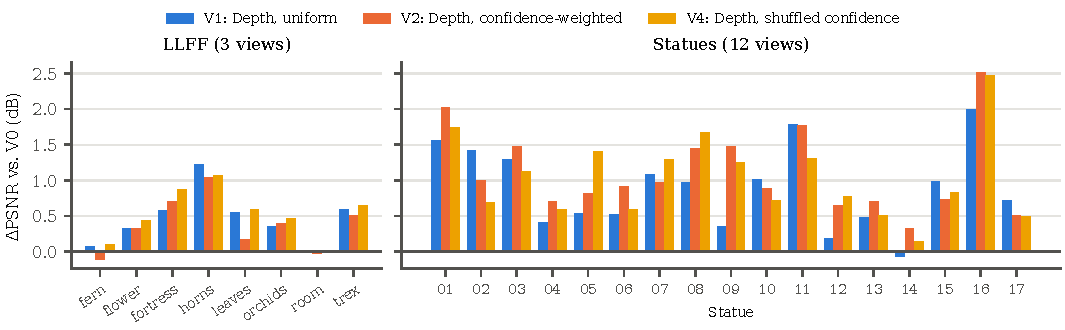
\includegraphics[width=\textwidth]{per_scene.pdf}
\caption{PSNR gain over the DropGaussian baseline per scene for the plain (V1), the confidence-weighted (V2) and the shuffled-confidence (V4) depth loss. LLFF: mean over three seeds; Statues: seed 0.}
\label{fig:perscene}
\end{figure*}

\subsection{Geometry}
Depth supervision also makes the reconstructed geometry more accurate at the held-out views (Table~\ref{tab:main}, AbsRel column): on LLFF, AbsRel falls from \LLFFVzeroabsrel{} for the baseline to \LLFFVoneabsrel{} with the plain loss (\LLFFVoneminusVzeroabsrelwins{} scenes, $p=\LLFFVoneminusVzeroabsrelp$). Here confidence weighting gives the lowest error of all variants (\LLFFVtwoabsrel{}; V2$-$V1 better in \LLFFVtwominusVoneabsrelwins{} scenes, $p=\LLFFVtwominusVoneabsrelp$), although the margin over the shuffled control is small and not significant (\LLFFVtwominusVfourabsrelwins{} scenes, $p=\LLFFVtwominusVfourabsrelp$). %STATUES-GEO
The geometry metric counts only pixels where the reference is opaque, which excludes much of the distant background; this matters for the explanation below.

\subsection{Is the confidence calibrated?}

\begin{table}[t]
\centering
\caption{Calibration of DA3 confidence against the reference depth, mean over scenes (number of scenes in brackets). AURG (depth): removing pixels farthest-first by the prior's own depth. $\rho_s(c,e)$: rank correlation of confidence and error; $|$depth: with the depth rank partialled out; $\rho_s(c,d)$: of confidence and depth.}
\label{tab:calib}
\footnotesize
\setlength{\tabcolsep}{3pt}
\begin{tabular}{@{}lcccccc@{}}
\toprule
 & AUSE$\downarrow$ & AURG$\uparrow$ & \makecell{AURG\\(depth)} & $\rho_s(c,e)$ & \makecell{$\rho_s(c,e)$\\$|$depth} & $\rho_s(c,d)$ \\
\midrule
LLFF (8) & 0.398 & 0.229 & -0.010 & -0.26 & -0.24 & -0.58 \\
Statues (17) & 0.381 & 0.261 & 0.050 & -0.24 & -0.30 & -0.84 \\
\bottomrule
\end{tabular}

\end{table}

\begin{figure}[t]
\centering
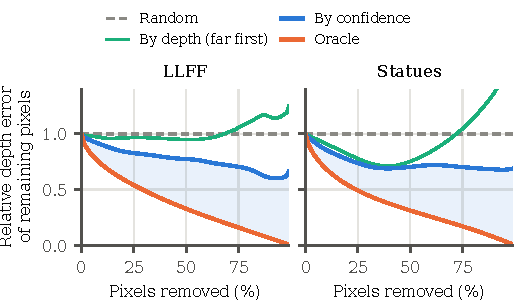
\includegraphics[width=\columnwidth]{sparsification.pdf}
\caption{Sparsification curves averaged over all training views: mean depth error of the pixels that remain when pixels are removed at random, by increasing confidence, farthest-first by predicted depth, or by decreasing true error (oracle). The shaded area is the AUSE.}
\label{fig:sparsification}
\end{figure}

Yes, partly (Table~\ref{tab:calib}, Fig.~\ref{fig:sparsification}). Removing the least confident pixels lowers the error of the rest in every LLFF scene (mean AURG \LLFFcalibaurg{}), but the confidence curve stays far from the oracle (AUSE \LLFFcalibause{}): confidence ranks errors much better than chance and much worse than perfect.

Because DA3 confidence falls with distance ($\rho_s(c,d)=\LLFFconfdepthall$ over all LLFF pixels and \Statuesconfdepthall{} over all statue pixels), a positive AURG could simply mean that far pixels are less accurate. The depth control rules this out: removing pixels farthest-first does no better than random on LLFF (AURG \LLFFcalibaurgdepth{}), confidence beats it in \LLFFcalibbeyonddepth{} scenes, and the confidence--error correlation survives partialling out depth ($\rho_s=\LLFFcalibpartial$). %STATUES-CALIB
The confidence therefore carries real information about where the prior is wrong.

\begin{figure*}[t]
\centering
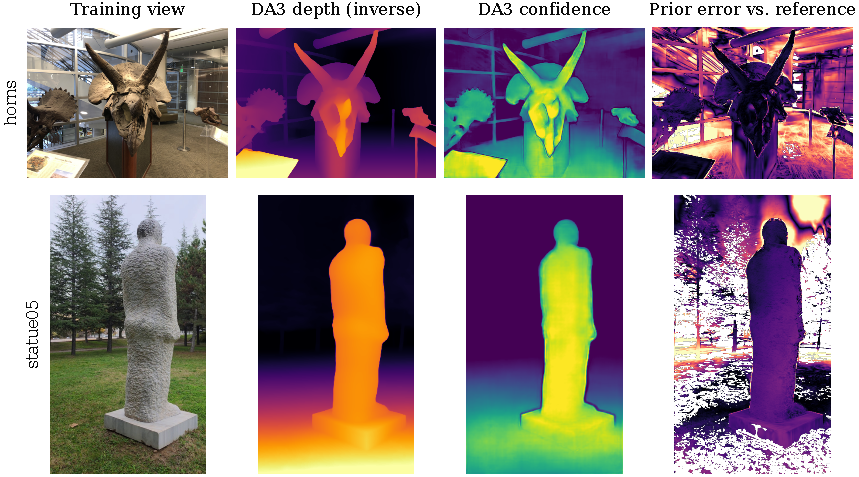
\includegraphics[width=\textwidth]{prior_error.pdf}
\caption{A training view, the DA3 depth and confidence for it, and the error of the (scale- and shift-aligned) DA3 depth against the reference, which is undefined (white) where the reference is not opaque. Low confidence covers the distant background as a whole, not only the pixels where the prior is wrong.}
\label{fig:prior}
\end{figure*}

\subsection{Why calibrated confidence does not help}
The two findings, an informative confidence and no gain from using it, are reconciled by \emph{where} the confidence-weighted loss puts its weight. Rank-normalised confidence gives the nearest third of each image (by predicted depth) a mean weight of \LLFFweightnear{} on LLFF and \Statuesweightnear{} on the statues, but the farthest third only \LLFFweightfar{} and \Statuesweightfar{} (Fig.~\ref{fig:prior}). V2 thus mostly removes depth supervision from the background, which is exactly the part of a sparse-view scene that few views constrain and where 3DGS forms floaters. The shuffled control V4 down-weights the same fraction of pixels, but uniformly over the image, so every region keeps on average half of its supervision. The ordering V3\,$<$\,V2\,$<$\,V4 in PSNR follows how much supervision reaches the background, not how accurately the remaining pixels are predicted.

Two further properties of the loss work in the same direction. First, the Pearson loss is invariant to scale and shift and compares only the shape of the depth map, so a prior that is wrong by a smooth, image-wide distortion still gives useful guidance; the errors that confidence detects are mostly local (depth edges, thin structures, sky) and matter little to a global correlation. Second, the geometry metric is restricted to pixels where the reference is opaque, which favours accurate nearby geometry; V2 is best there, while PSNR also scores the background, where V2 is weakest. For sparse-view 3DGS with a correlation loss, \emph{coverage} of the depth supervision matters more than its accuracy.

\subsection{Sensitivity to the depth weight}
%SENSITIVITY

\subsection{Qualitative results}
Fig.~\ref{fig:qualitative} shows test views from the scenes with the largest and the smallest gain of V1 over the baseline on each benchmark (\qualrows). Depth supervision mainly removes floaters and fills the background with coherent surfaces; differences between V1 and V2 are hard to see. Fly-through videos of trained models are in the repository (\texttt{demo/}).

\begin{figure*}[t]
\centering
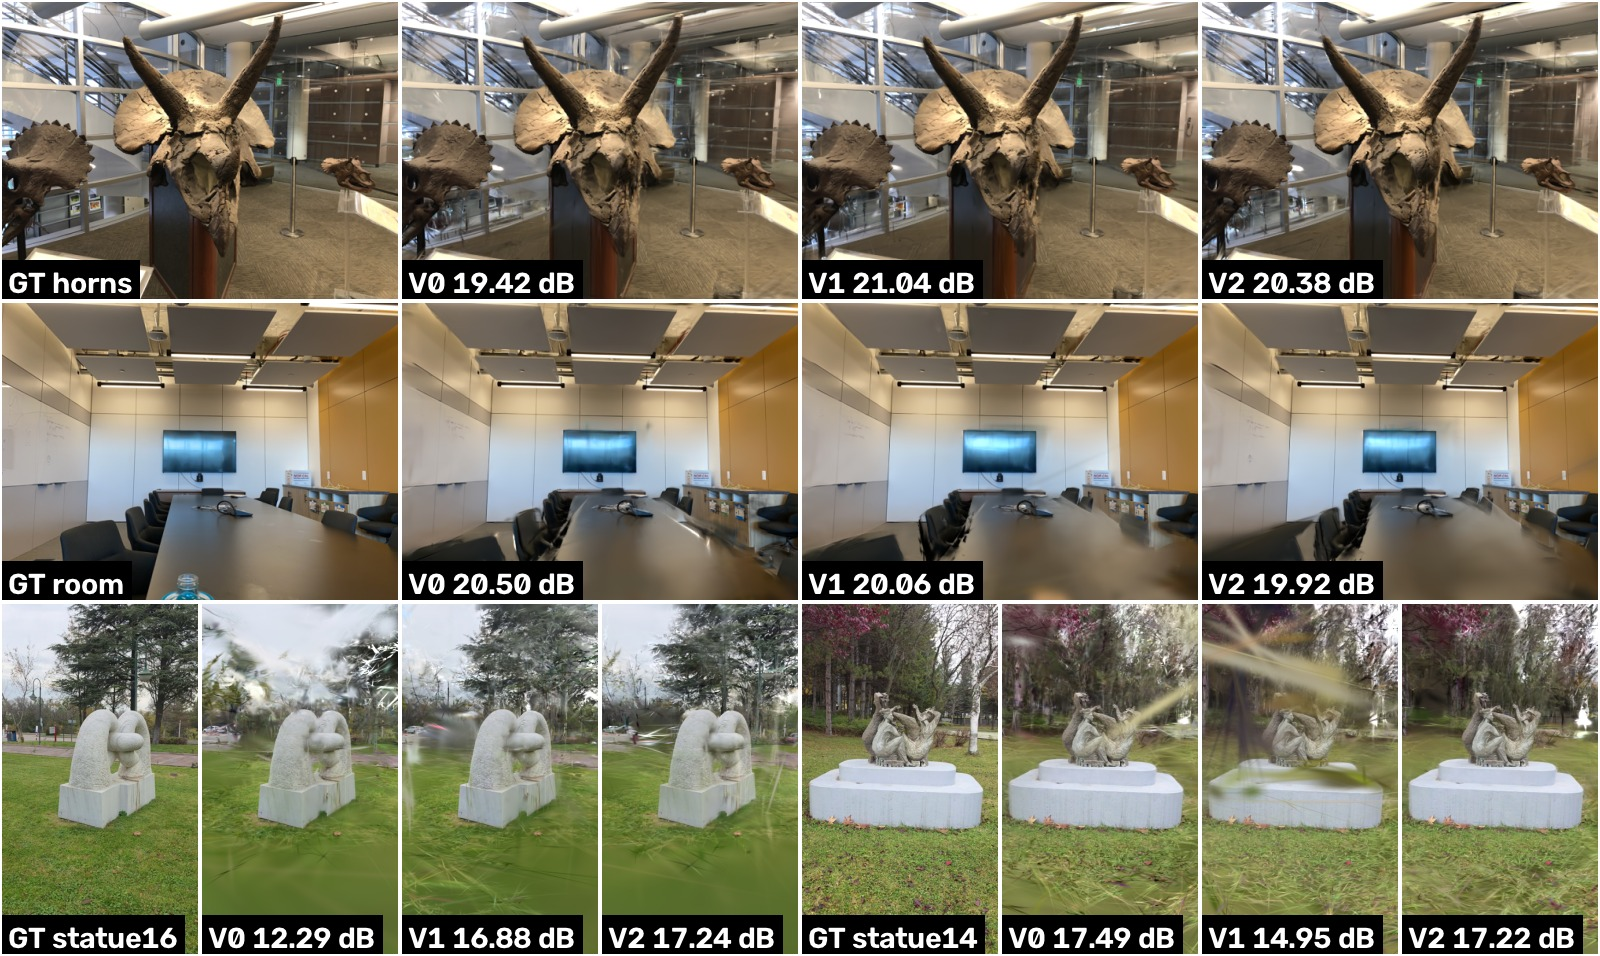
\includegraphics[width=\textwidth]{qualitative.jpg}
\caption{Test views (seed 0): ground truth, the baseline (V0), the plain depth loss (V1) and the confidence-weighted loss (V2), with per-image PSNR. Rows: \qualrows.}
\label{fig:qualitative}
\end{figure*}

\subsection{Cost}
Depth supervision needs one DA3 forward pass per scene (seconds) and a second rasterisation per iteration. The median training time rises from \LLFFVzerominutes{} to \LLFFVoneminutes{} minutes on LLFF %STATUES-COST
; the weighting itself costs nothing measurable.

\section{Discussion and Limitations}
\textbf{Reference, not ground truth.} The geometry and calibration analyses use reconstructions from all non-test views as reference. They are well constrained where views overlap but can be wrong at the image borders, on thin structures and on reflective surfaces, and they exclude non-opaque background. Errors of the reference count as errors of the prior, which would make the confidence look worse calibrated than it is, not better.

\textbf{Scope.} We test one depth model (DA3-Large), one baseline, one loss form (Pearson) and one depth weight, fixed on two LLFF scenes. The statues are trained with a single seed. Weighting schemes that keep coverage, for example normalising confidence within depth bands, or using confidence to modulate a scale-aware loss rather than a correlation, are natural next steps that our analysis suggests but does not test.

\textbf{Failure cases.} %FAILURES

\section{Conclusion}
Depth supervision from a current multi-view depth foundation model is a reliable improvement for sparse-view 3D Gaussian Splatting: it adds about half a decibel on LLFF %STATUES-CONCL
 and makes the reconstructed geometry measurably more accurate, at the price of one forward pass per scene and a second rasterisation per step. Weighting that supervision by the model's own confidence, however, does not improve image quality, even though the confidence does indicate where the predicted depth is wrong, beyond what distance alone explains. The reason is that the confidence is low over entire distant regions, and removing supervision there costs more than the errors it avoids; a shuffled-confidence control that keeps the same weights but spreads them evenly is better in every LLFF scene.

\textbf{Applications.} The pipeline turns a 30--60\,s phone video into a navigable 3D model from a dozen frames, which suits quick documentation of cultural-heritage objects such as the Hacettepe statues, site and infrastructure inspection with few passes, and robots that see a place only briefly. Our results suggest that such systems should use depth priors, and should not trust confidence-based masking to make them safer.
